% Options for packages loaded elsewhere
\PassOptionsToPackage{unicode=true}{hyperref}
\PassOptionsToPackage{hyphens}{url}
%
\documentclass[
  letterpaper,
  twocolumn]{article}
\usepackage{lmodern}
\usepackage{amssymb,amsmath}
\usepackage{ifxetex,ifluatex}
\ifnum 0\ifxetex 1\fi\ifluatex 1\fi=0 % if pdftex
  \usepackage[T1]{fontenc}
  \usepackage[utf8]{inputenc}
  \usepackage{textcomp} % provides euro and other symbols
\else % if luatex or xelatex
  \usepackage{unicode-math}
  \defaultfontfeatures{Scale=MatchLowercase}
  \defaultfontfeatures[\rmfamily]{Ligatures=TeX,Scale=1}
\fi
% Use upquote if available, for straight quotes in verbatim environments
\IfFileExists{upquote.sty}{\usepackage{upquote}}{}
\IfFileExists{microtype.sty}{% use microtype if available
  \usepackage[]{microtype}
  \UseMicrotypeSet[protrusion]{basicmath} % disable protrusion for tt fonts
}{}
\makeatletter
\@ifundefined{KOMAClassName}{% if non-KOMA class
  \IfFileExists{parskip.sty}{%
    \usepackage{parskip}
  }{% else
    \setlength{\parindent}{0pt}
    \setlength{\parskip}{6pt plus 2pt minus 1pt}}
}{% if KOMA class
  \KOMAoptions{parskip=half}}
\makeatother
\usepackage{xcolor}
\IfFileExists{xurl.sty}{\usepackage{xurl}}{} % add URL line breaks if available
\IfFileExists{bookmark.sty}{\usepackage{bookmark}}{\usepackage{hyperref}}
\hypersetup{
  pdftitle={Bee Movie},
  pdfauthor={Barry B. Benson},
  hidelinks,
}
\urlstyle{same} % disable monospaced font for URLs
\usepackage[margin=1in]{geometry}
\usepackage{color}
\usepackage{fancyvrb}
\newcommand{\VerbBar}{|}
\newcommand{\VERB}{\Verb[commandchars=\\\{\}]}
\DefineVerbatimEnvironment{Highlighting}{Verbatim}{commandchars=\\\{\}}
% Add ',fontsize=\small' for more characters per line
\newenvironment{Shaded}{}{}
\newcommand{\AlertTok}[1]{\textcolor[rgb]{1.00,0.00,0.00}{\textbf{#1}}}
\newcommand{\AnnotationTok}[1]{\textcolor[rgb]{0.38,0.63,0.69}{\textbf{\textit{#1}}}}
\newcommand{\AttributeTok}[1]{\textcolor[rgb]{0.49,0.56,0.16}{#1}}
\newcommand{\BaseNTok}[1]{\textcolor[rgb]{0.25,0.63,0.44}{#1}}
\newcommand{\BuiltInTok}[1]{#1}
\newcommand{\CharTok}[1]{\textcolor[rgb]{0.25,0.44,0.63}{#1}}
\newcommand{\CommentTok}[1]{\textcolor[rgb]{0.38,0.63,0.69}{\textit{#1}}}
\newcommand{\CommentVarTok}[1]{\textcolor[rgb]{0.38,0.63,0.69}{\textbf{\textit{#1}}}}
\newcommand{\ConstantTok}[1]{\textcolor[rgb]{0.53,0.00,0.00}{#1}}
\newcommand{\ControlFlowTok}[1]{\textcolor[rgb]{0.00,0.44,0.13}{\textbf{#1}}}
\newcommand{\DataTypeTok}[1]{\textcolor[rgb]{0.56,0.13,0.00}{#1}}
\newcommand{\DecValTok}[1]{\textcolor[rgb]{0.25,0.63,0.44}{#1}}
\newcommand{\DocumentationTok}[1]{\textcolor[rgb]{0.73,0.13,0.13}{\textit{#1}}}
\newcommand{\ErrorTok}[1]{\textcolor[rgb]{1.00,0.00,0.00}{\textbf{#1}}}
\newcommand{\ExtensionTok}[1]{#1}
\newcommand{\FloatTok}[1]{\textcolor[rgb]{0.25,0.63,0.44}{#1}}
\newcommand{\FunctionTok}[1]{\textcolor[rgb]{0.02,0.16,0.49}{#1}}
\newcommand{\ImportTok}[1]{#1}
\newcommand{\InformationTok}[1]{\textcolor[rgb]{0.38,0.63,0.69}{\textbf{\textit{#1}}}}
\newcommand{\KeywordTok}[1]{\textcolor[rgb]{0.00,0.44,0.13}{\textbf{#1}}}
\newcommand{\NormalTok}[1]{#1}
\newcommand{\OperatorTok}[1]{\textcolor[rgb]{0.40,0.40,0.40}{#1}}
\newcommand{\OtherTok}[1]{\textcolor[rgb]{0.00,0.44,0.13}{#1}}
\newcommand{\PreprocessorTok}[1]{\textcolor[rgb]{0.74,0.48,0.00}{#1}}
\newcommand{\RegionMarkerTok}[1]{#1}
\newcommand{\SpecialCharTok}[1]{\textcolor[rgb]{0.25,0.44,0.63}{#1}}
\newcommand{\SpecialStringTok}[1]{\textcolor[rgb]{0.73,0.40,0.53}{#1}}
\newcommand{\StringTok}[1]{\textcolor[rgb]{0.25,0.44,0.63}{#1}}
\newcommand{\VariableTok}[1]{\textcolor[rgb]{0.10,0.09,0.49}{#1}}
\newcommand{\VerbatimStringTok}[1]{\textcolor[rgb]{0.25,0.44,0.63}{#1}}
\newcommand{\WarningTok}[1]{\textcolor[rgb]{0.38,0.63,0.69}{\textbf{\textit{#1}}}}
\usepackage{graphicx,grffile}
\makeatletter
\def\maxwidth{\ifdim\Gin@nat@width>\linewidth\linewidth\else\Gin@nat@width\fi}
\def\maxheight{\ifdim\Gin@nat@height>\textheight\textheight\else\Gin@nat@height\fi}
\makeatother
% Scale images if necessary, so that they will not overflow the page
% margins by default, and it is still possible to overwrite the defaults
% using explicit options in \includegraphics[width, height, ...]{}
\setkeys{Gin}{width=\maxwidth,height=\maxheight,keepaspectratio}
\setlength{\emergencystretch}{3em} % prevent overfull lines
\providecommand{\tightlist}{%
  \setlength{\itemsep}{0pt}\setlength{\parskip}{0pt}}
\setcounter{secnumdepth}{-\maxdimen} % remove section numbering
% Redefines (sub)paragraphs to behave more like sections
\ifx\paragraph\undefined\else
  \let\oldparagraph\paragraph
  \renewcommand{\paragraph}[1]{\oldparagraph{#1}\mbox{}}
\fi
\ifx\subparagraph\undefined\else
  \let\oldsubparagraph\subparagraph
  \renewcommand{\subparagraph}[1]{\oldsubparagraph{#1}\mbox{}}
\fi

% Set default figure placement to htbp
\makeatletter
\def\fps@figure{htbp}
\makeatother


\title{Bee Movie}
\usepackage{etoolbox}
\makeatletter
\providecommand{\subtitle}[1]{% add subtitle to \maketitle
  \apptocmd{\@title}{\par {\large #1 \par}}{}{}
}
\makeatother
\subtitle{Honey Just Got Funny}
\author{Barry B. Benson}
\date{November 2, 2007}

\begin{document}
\maketitle
\begin{abstract}
According to all known laws of aviation, there is no way a bee should be
able to fly (Smith et al. (2007)). Its wings are too small to get its
fat little body off the ground. The bee, of course, flies anyway because
\textbf{bees don't care what humans think is impossible}.
\end{abstract}

\hypertarget{unbeelievable}{%
\section{Unbeelievable}\label{unbeelievable}}

Yellow, black. Yellow, black. Yellow, black. Yellow, black. Ooh, black
and yellow! Let's shake it up a little. Barry! Breakfast is ready!
Coming! Hang on a second. Hello? - Barry? - Adam? - Can you believe this
is happening? - I can't. I'll pick you up. Looking sharp. Use the
stairs. Your father paid good money for those. Sorry. I'm excited.
Here's the graduate.

\begin{itemize}
\tightlist
\item
  We're very proud of you, son.
\item
  A perfect report card, all B's. Very proud.
\item
  Ma! I got a thing going here.
\end{itemize}

You got lint on your fuzz. - Ow! That's me! - Wave to us! We'll be in
row 118,000. - Bye! Barry, I told you, stop flying in the house!

\begin{figure}
\centering
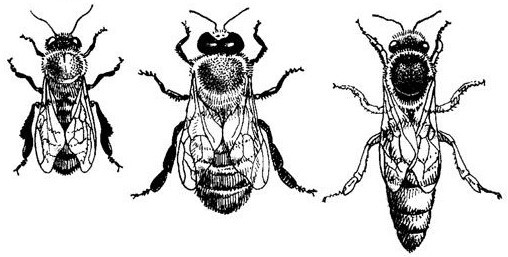
\includegraphics{assets/bee-castes.jpg}
\caption{Bee Castes: worker, drone, queen (from left to right)}
\end{figure}

Hey, Adam. - Hey, Barry. - Is that fuzz gel? - A little. Special day,
graduation. Never thought I'd make it. Three days grade school, three
days high school. Those were awkward. Three days college. I'm glad I
took a day and hitchhiked around the hive. You did come back different.
- Hi, Barry. - Artie, growing a mustache? Looks good. - Hear about
Frankie? - Yeah. - You going to the funeral? - No, I'm not going.
\emph{Everybody knows, sting someone, you die}. Don't waste it on a
squirrel. Such a hothead. I guess he could have just gotten out of the
way.

\[ \frac{F}{A} = \eta \frac{\Delta v_x}{\Delta z} \]

I love this incorporating an amusement park into our day. That's why we
don't need vacations. Boy, quite a bit of pomp\ldots{} under the
circumstances. - Well, Adam, today we are men. - We are! - Bee-men. -
Amen! Hallelujah! Students, faculty, distinguished bees, please welcome
Dean Buzzwell. Welcome, New Hive City graduating class of\ldots{}
\ldots9:15. That concludes our ceremonies. And begins your career at
Honex Industries! Will we pick our job today? I heard it's just
orientation.

\hypertarget{unacceptable-beehavior}{%
\subsection{Unacceptable Beehavior}\label{unacceptable-beehavior}}

Heads up! Here we go. Keep your hands and antennas inside the tram at
all times. - Wonder what it'll be like? - A little scary. Welcome to
Honex, a division of Honesco and a part of the Hexagon Group. This is
it! Wow. Wow.
\texttt{We\ know\ that\ you,\ as\ a\ bee,\ have\ worked\ your\ whole\ life\ to\ get\ to\ the\ point\ where\ you\ can\ work\ for\ your\ whole\ life}.
Honey begins when our valiant Pollen Jocks bring the nectar to the hive.
Our top-secret formula is automatically color-corrected, scent-adjusted
and bubble-contoured into this soothing sweet syrup with its distinctive
golden glow you know as\ldots{} Honey!

\begin{Shaded}
\begin{Highlighting}[]
\NormalTok{l }\OperatorTok{=} \StringTok{"That girl was hot. She's my cousin!"}
\BuiltInTok{print}\NormalTok{(}\StringTok{"}\SpecialCharTok\NormalTok{ l)}
\end{Highlighting}
\end{Shaded}

Yes, we're all cousins. - Right. You're right.

\hypertarget{beeware-honex}{%
\section{Beeware Honex}\label{beeware-honex}}

At \href{https://www.amazon.com/}{Honex}, we constantly strive to
improve every aspect of bee existence. These bees are stress-testing a
new helmet technology. - What do you think he makes? - Not enough. Here
we have our latest advancement, the Krelman. - What does that do? -
Catches that little strand of honey that hangs after you pour it. Saves
us millions. Can anyone work on the Krelman? Of course.

Most bee jobs are small ones. But bees know that every small job, if
it's done well, means a lot. But choose carefully because you'll stay in
the job you pick for the rest of your life. The same job the rest of
your life? I didn't know that. What's the difference? You'll be happy to
know that bees, as a species, haven't had one day off in 27 million
years. \textbf{So you'll just work us to death? We'll sure try}. Wow!
That blew my mind! ``What's the difference?'' How can you say that?
\emph{One job forever? That's an insane choice to have to make}. I'm
relieved. Now we only have to make one decision in life.

But, Adam, how could they never have told us that? Why would you
question anything? We're bees. We're the most perfectly functioning
society on Earth. You ever think maybe things work a little too well
here? Like what? Give me one example. I don't know. But you know what
I'm talking about. Please clear the gate. Royal Nectar Force on
approach. Wait a second. Check it out.

\hypertarget{what-is-all-this-buzz-about}{%
\subsection{What Is All This Buzz
About?}\label{what-is-all-this-buzz-about}}

Hey, those are Pollen Jocks! - Wow. I've never seen them this close.
They know what it's like outside the hive. Yeah, but some don't come
back. - Hey, Jocks! - Hi, Jocks! You guys did great! You're monsters!
You're sky freaks! I love it! I love it! - I wonder where they were. - I
don't know. Their day's not planned. Outside the hive, flying who knows
where, doing who knows what. You can't just decide to be a Pollen Jock.
You have to be bred for that. Right. Look. That's more pollen than you
and I will see in a lifetime. It's just a status symbol. Bees make too
much of it. Perhaps. Unless you're wearing it and the ladies see you
wearing it. Those ladies? Aren't they our cousins too? Distant. Distant.
Look at these two. - Couple of Hive Harrys. - Let's have fun with them.
It must be dangerous being a Pollen Jock. Yeah.

\begin{enumerate}
\def\labelenumi{\arabic{enumi}.}
\tightlist
\item
  Once a bear pinned me against a mushroom!
\item
  He had a paw on my throat, and with the other, he was slapping me!
\item
  Oh, my! - I never thought I'd knock him out.
\end{enumerate}

What were you doing during this? Trying to alert the authorities. I can
autograph that. A little gusty out there today, wasn't it, comrades?
Yeah. Gusty. We're hitting a sunflower patch six miles from here
tomorrow. - Six miles, huh? - Barry! A puddle jump for us, but maybe
you're not up for it. - Maybe I am. - You are not! We're going 0900 at
J-Gate. What do you think, buzzy-boy? Are you bee enough? I might be. It
all depends on what 0900 means. Hey, Honex!

\hypertarget{bee-yourself}{%
\subsection{Bee Yourself}\label{bee-yourself}}

Dad, you surprised me. You decide what you're interested in? - Well,
there's a lot of choices. - But you only get one. Do you ever get bored
doing the same job every day? Son, let me tell you about stirring. You
grab that stick, and you just move it around, and you stir it around.
You get yourself into a rhythm. It's a beautiful thing. You know, Dad,
the more I think about it, maybe the honey field just isn't right for
me. You were thinking of what, making balloon animals? That's a bad job
for a guy with a stinger. Janet, your son's not sure he wants to go into
honey! - Barry, you are so funny sometimes. - I'm not trying to be
funny. You're not funny! You're going into honey. Our son, the stirrer!
- You're gonna be a stirrer? - No one's listening to me! Wait till you
see the sticks I have. I could say anything right now. I'm gonna get an
ant tattoo! Let's open some honey and celebrate! Maybe I'll pierce my
thorax. Shave my antennae. Shack up with a grasshopper. Get a gold tooth
and call everybody ``dawg''! I'm so proud. - We're starting work today!
- Today's the day. Come on! All the good jobs will be gone. Yeah, right.
Pollen counting, stunt bee, pouring, stirrer, front desk, hair
removal\ldots{} - Is it still available? - Hang on. Two left! One of
them's yours! Congratulations! Step to the side. - What'd you get? -
Picking crud out. Stellar! Wow! Couple of newbies? Yes, sir!

Our first day! We are ready! Make your choice. - You want to go first? -
No, you go. Oh, my. What's available? Restroom attendant's open, not for
the reason you think. - Any chance of getting the Krelman? - Sure,
you're on. I'm sorry, the Krelman just closed out. Wax monkey's always
open. The Krelman opened up again. What happened? A bee died.

\hypertarget{references}{%
\section*{References}\label{references}}
\addcontentsline{toc}{section}{References}

\hypertarget{refs}{}
\leavevmode\hypertarget{ref-beeMovieId}{}%
Smith, Simon, Steve Hickner, Jerry Seinfeld, and others. 2007. ``There
Is No Way a Bee Should Be Able to Fly.'' \emph{Honey} 420 (7): 91--92.

\end{document}
